\documentclass[10pt]{article}
\usepackage[a4paper,margin=22mm]{geometry}
\usepackage[T1]{fontenc}
\usepackage[utf8]{inputenc}
\usepackage{lmodern,amsmath,amssymb,graphicx,float,fancyhdr,xcolor}
\usepackage{fancyvrb,etoolbox}
\BeforeBeginEnvironment{verbatim}{\par\noindent\begin{minipage}{\linewidth}}
\AfterEndEnvironment{verbatim}{\end{minipage}\par}
\usepackage[unicode,hidelinks]{hyperref}
\DeclareUnicodeCharacter{2192}{\ensuremath{\rightarrow}}
\providecommand{\textt}[1]{\texttt{#1}}
\providecommand{\tightlist}{\setlength{\itemsep}{0pt}\setlength{\parskip}{0pt}}
\setlength{\parindent}{0pt}
\setlength{\parskip}{0.6em}
\setlength{\headheight}{41pt}
\setlength{\emergencystretch}{3em}
\pagestyle{fancy}
\lhead{
\includegraphics[width=2.5cm]{edem_logo.jpg}}
\rhead{Computer Science -- Solved rehearsal}
\cfoot{\thepage}
\let\OldSection\section
\renewcommand{\section}{\clearpage\OldSection}
\begin{document}
\begin{center}
{\LARGE\bfseries Computer Science\\Partial exam rehearsal -- Solved version\par}
\vspace{1em}
IGE -- 1st Year\\Class practice
\end{center}
\textbf{Suggested duration:} 1 hour 45 minutes, followed by class discussion.

Try each question before reading its solution. For multiple-choice questions, choose one answer and justify it. Questions and solutions are in English.

\textbf{Content.} This rehearsal covers three units. Unit 1 focuses on binary representation, CPU instructions and register states (2 points, 20\%). Unit 2 covers Python imports, numeric operations, Boolean conditions, \texttt{if-elif-else}, loops and lists (3 points, 30\%). Unit 3 covers Arduino programming, error detection, digital inputs and outputs, and an LCD scoreboard (5 points, 50\%). These weights are indicative for this academic year and should be used as a guide when preparing for the exam.

\section*{Unit 1 Problems (2.0 points total)}

\subsection*{Q1 - CPU execution}
A processor has four registries, labeled R0, R1, R2, and R3 and the following set of operation codes: 
\begin{enumerate}
    \item \texttt{0001} Addition
    \item \texttt{0010} Substraction
    \item \texttt{1100} Multiplication
    \item \texttt{1101} Integer Division
    \item \texttt{1110} Modulo (reminder after Integer division)
\end{enumerate}
The 10-bit instruction is formatted as follows. 

\texttt{Opcode(4) | Dest(2) | Src1(2) | Src2(2)}

For example, the instruction \texttt{1110 00 01 10} means "calculate the reminder after Integer division of the value of registry R1 divided by the value of registry R2 (R1 modulo R2), and store the value in registry R0".

The initial value in the registers are in table \ref{tab:initial_state}: 

\begin{table}[H]
    \begin{tabular}{ll}
        R0 & \textt{0b1011}\\
        R1 & \textt{0b1000}\\
        R2 & \textt{0b0010}\\
        R3 & \textt{0b0000} \\ 
    \end{tabular}
    \caption{Initial states}
    \label{tab:initial_state}
\end{table}



Answer the following questions: 
\begin{enumerate}
    \item Convert to decimal the values in registry (prefixed with \verb|0b|). \textbf{(0.5 pts)}
    
    \textbf{Solution:}
    \begin{itemize}
        \item R0 = 0b1011 = 11
        \item R1 = 0b1000 = 8
        \item R2 = 0b0010 = 2
        \item R3 = 0b0000 = 0
    \end{itemize}
    \item Write the instruction to add the values in registries R1 and R2 and store it back in registry R2. This instruction will be instruction 1. \textbf{(0.2 pts)}\\
    
    \textbf{Solution:}
    
    Opcode for ADD = \texttt{0001}\\
    Dest = R2 = \texttt{10}\\
    Src1 = R1 = \texttt{01}\\
    Src2 = R2 = \texttt{10}\\
    
    Final instruction:
    \[
    \texttt{0001\,10\,01\,10}
    \]

    \item Consider the following instructions:
    \begin{itemize}
        \item Instruction 2: 0010000001
        \item Instruction 3: 1110110100
    \end{itemize}
    Explain what every instruction will do.(0.3 pts)

    \textbf{Solution:}
    \begin{itemize}
        \item Instruction 2: \texttt{0010 00 00 01}  
        Opcode 0010 = subtraction.  
        R0 = R0 - R1.
        
        \item Instruction 3: \texttt{1110 11 01 00}  
        Opcode 1110 = modulo.  
        R3 = R1 mod R0.
    \end{itemize}
    \textbf{(0.3 pts)}
    \item Using the initial state, apply instruction1, instruction2 and instruction3. Show the state
of the registers after the execution of every instruction. \textbf{(1 pts)}      

\textbf{Solution:}
\begin{enumerate}
\item \textbf{Instruction 1: ADD R1 and R2 → R2}  

R2 = 8 + 2 = 10  
R2 = \texttt{0b1010}

Registers:  
\[
\begin{aligned}
R0 &= 11\;(\texttt{0b1011})\\
R1 &= 8\;(\texttt{0b1000})\\
R2 &= 10\;(\texttt{0b1010})\\
R3 &= 0\;(\texttt{0b0000})
\end{aligned}
\]

\item \textbf{Instruction 2: SUB R0 = R0 - R1}  

R0 = 11 - 8 = 3  
R0 = \texttt{0b0011}

Registers:  
\[
\begin{aligned}
R0 &= 3\;(\texttt{0b0011})\\
R1 &= 8\;(\texttt{0b1000})\\
R2 &= 10\;(\texttt{0b1010})\\
R3 &= 0\;(\texttt{0b0000})
\end{aligned}
\]

\item \textbf{Instruction 3: MOD R3 = R1 mod R0}  

R3 = 8 mod 3 = 2  
R3 = \texttt{0b0010}

Final registers:  
\[
\begin{aligned}
R0 &= 3\;(\texttt{0b0011})\\
R1 &= 8\;(\texttt{0b1000})\\
R2 &= 10\;(\texttt{0b1010})\\
R3 &= 2\;(\texttt{0b0010})
\end{aligned}
\]
\end{enumerate}

\end{enumerate}


\section*{Unit 2 -- Python (3 points total)}
\subsection*{Python Q1 -- Scenario 4 -- Requesting a concise import (0.375 pt)}
A financial analyst only needs \texttt{sqrt()} from the \texttt{math}
module and wants to call it without the \texttt{math.} prefix. Which
option meets the requirement?

A. \texttt{import\ math} followed by \texttt{math.sqrt(81)}\\
B. \texttt{import\ math\ as\ sqrt} followed by \texttt{sqrt(81)}\\
C. \texttt{from\ math\ import\ sqrt} followed by \texttt{sqrt(81)}\\
D. \texttt{from\ sqrt\ import\ math} followed by \texttt{sqrt(81)}

\textbf{Your choice:}\\
\textbf{Which name becomes available?}

\subsubsection*{Solution}
\textbf{Answer: C.} \texttt{from\ math\ import\ sqrt} imports the
function under the name \texttt{sqrt}, so \texttt{sqrt(81)} returns
\texttt{9.0}. A retains the prefix; B binds the module to \texttt{sqrt}
and then attempts to call a module; D reverses the module and function
names.

\textbf{Marking:} correct option, 0.125; justification using the
requirement and explaining a distractor or counterexample, 0.25.

\subsection*{Python Q2 -- Scenario 2 -- Packing devices (0.375 pt)}
A warehouse must pack 137 devices into boxes that hold 12 devices each.
The manager needs the number of complete boxes and unpacked devices.
Which solution is most appropriate?

\begin{enumerate}
\def\labelenumi{\Alph{enumi}.}
\tightlist
\item
\end{enumerate}

\begin{verbatim}
boxes = 137 / 12
remaining = 137 / 12
\end{verbatim}

\begin{enumerate}
\def\labelenumi{\Alph{enumi}.}
\setcounter{enumi}{1}
\tightlist
\item
\end{enumerate}

\begin{verbatim}
boxes = 137 // 12
remaining = 137 % 12
\end{verbatim}

\begin{enumerate}
\def\labelenumi{\Alph{enumi}.}
\setcounter{enumi}{2}
\tightlist
\item
\end{enumerate}

\begin{verbatim}
boxes = 137 % 12
remaining = 137 // 12
\end{verbatim}

\begin{enumerate}
\def\labelenumi{\Alph{enumi}.}
\setcounter{enumi}{3}
\tightlist
\item
\end{enumerate}

\begin{verbatim}
boxes = int(137 / 12)
remaining = 137 - 12
\end{verbatim}

\textbf{Your choice and justification:}

\subsubsection*{Solution}
\textbf{Answer: B.} Integer division gives \texttt{11} complete boxes
and modulo gives \texttt{5} remaining devices:
\texttt{137\ =\ 11\ *\ 12\ +\ 5}. A uses ordinary division; C swaps the
results; D subtracts only one box capacity.

\textbf{Marking:} correct option, 0.125; justification using the
requirement and explaining a distractor or counterexample, 0.25.

\clearpage
\subsection*{Python Q3 -- Scenario 4 -- Secure document access (0.375 pt)}
A user may open a confidential document when they have permission and
their account is not suspended. The following code illustrates how the
condition will be used. Replace \texttt{<condition>} with one of the
options below. Which condition states the requirement most directly?

\begin{verbatim}
has_permission = True
account_suspended = False

if <condition>:
    print("Access granted")
else:
    print("Access denied")
\end{verbatim}

A. \texttt{has\_permission\ or\ not\ account\_suspended}\\
B. \texttt{has\_permission\ and\ not\ account\_suspended}\\
C. \texttt{not\ has\_permission\ and\ account\_suspended}\\
D. \texttt{has\_permission\ and\ account\_suspended}

\textbf{Your choice and a test that should deny access:}

\subsubsection*{Solution}
\textbf{Answer: B.} Both requirements must hold:
\texttt{has\_permission\ and\ not\ account\_suspended}. Access must be
denied when permission is \texttt{True} and suspension is \texttt{True}.
It must also be denied when permission is \texttt{False}. Option A could
grant access without permission. With the sample values, the corrected
code prints \texttt{Access granted}.

\textbf{Marking:} correct option, 0.125; justification using the
requirement and explaining a distractor or counterexample, 0.25.

\subsection*{Python Q4 -- B7. Diagnosing an index error (0.375 pt)}
An AI assistant generates the following loop and Python raises
\texttt{IndexError} on the last iteration:

\begin{verbatim}
for index in range(len(values) + 1):
    print(values[index])
\end{verbatim}

Which explanation is most accurate?

A. Lists cannot be used inside \texttt{for} loops.

B. \texttt{range()} includes its stop value.

C. The \texttt{+\ 1} creates an index equal to the list length, which is
outside the valid range.

D. The loop must begin at index \texttt{1}.

\subsubsection*{Solution}
\textbf{Answer: C.} For a list of length \texttt{n}, valid indices are
\texttt{0} to \texttt{n\ -\ 1}. \texttt{range(n\ +\ 1)} also produces
\texttt{n}, causing the error. \texttt{range()} excludes its stop value,
so B is false. The correct header is\\
\texttt{for\ index\ in\ range(len(values)):}.

\textbf{Marking:} correct option, 0.125; justification using the
requirement and explaining a distractor or counterexample, 0.25.

\clearpage
\subsection*{Python Q5 -- A7. Prioritise outcomes (0.75 pt)}
A support request should receive exactly one classification:
\begin{enumerate}
\item \texttt{"Critical"} when the service is unavailable.
\item \texttt{"High"} when data may be lost.
\item \texttt{"Medium"} when response time exceeds 5 seconds.
\item \texttt{"Normal"} otherwise.
\end{enumerate}
Implement the policy with \texttt{if-elif-else}. Create a case where several
conditions are true and explain why only one branch runs.

\begin{verbatim}
service_unavailable = False
possible_data_loss = True
response_time = 8.2

# Implement and print the classification here.
\end{verbatim}

\subsubsection*{Solution}
\begin{verbatim}
service_unavailable = False
possible_data_loss = True
response_time = 8.2

if service_unavailable:
    classification = "Critical"
elif possible_data_loss:
    classification = "High"
elif response_time > 5:
    classification = "Medium"
else:
    classification = "Normal"

print(classification)
\end{verbatim}
\textbf{Output:} \texttt{High}.

Both possible data loss and a response time above 5 seconds apply in the
supplied case. Python executes only the first matching branch in the
\texttt{if-elif-else} chain, so the higher-priority classification wins.
If \texttt{service\_unavailable} is changed to \texttt{True}, all three
conditions hold and the output is \texttt{Critical}.

When both Boolean values are \texttt{False}, a response time of
\texttt{8.2} produces \texttt{Medium}, while exactly \texttt{5} produces
\texttt{Normal}: the rule says ``exceeds'', not ``at least''.

\textbf{Marking:} correctly ordered \texttt{if-elif-else} chain, 0.25;
correct conditions, classifications and output, 0.25; a case with several
true conditions and explanation of branch priority, 0.25.

\clearpage
\subsection*{Python Q6 -- A5. Preserve a running series (0.75 pt)}
A new online service begins with \texttt{200} registered users (stored in
\texttt{initial\_users}). A list contains the new users gained each week
(\texttt{new\_users\_by\_week} stores the new users for each week).

Create \texttt{total\_users\_by\_week} so that it contains the initial
total followed by the total after every week.

\begin{verbatim}
initial_users = 200
new_users_by_week = [25, 30, 20, 35]
total_users = initial_users
total_users_by_week = [initial_users]

# Update total_users for every week.
# Preserve every updated total in total_users_by_week.

print(total_users_by_week)
# Expected: [200, 225, 255, 275, 310]
\end{verbatim}

\subsubsection*{Solution}
\begin{verbatim}
initial_users = 200
new_users_by_week = [25, 30, 20, 35]
total_users = initial_users
total_users_by_week = [initial_users]

for new_users in new_users_by_week:
    total_users = total_users + new_users
    total_users_by_week.append(total_users)

print(total_users_by_week)
\end{verbatim}

\textbf{Output:} \texttt{{[}200,\ 225,\ 255,\ 275,\ 310{]}}.

The running total is \texttt{225}, \texttt{255}, \texttt{275} and
\texttt{310} after weeks 1--4. Initialise the accumulator before the
loop and append inside it to preserve every updated total. The initial
\texttt{200} remains the first element. With no new weeks, the result is
\texttt{{[}200{]}}.

\textbf{Marking:} initial state, 0.25; accumulation, 0.25; storing each
total and correct result, 0.25.
\section*{Unit 3 Problems (5 points total)}

\subsection*{Q1 — Error Detection \& Correction (1.5)}
Consider the following code, it contains several syntax/logic errors.
\begin{verbatim}
const int led1 = 11
const int led2 = 2;
const int btn = 11;

void setup() {
    pinMode(led1, OUTPUT)
    pinMode(led2, OUTPUT);
    pinMode(btn, OUTPUT);
}

void setup() {
if (digitalRead(btn) = HIGH) {
    pattern = !pattern;
    }
    if (pattern = true) {
        digitalWrite(led1, HIGH);
        digitalWrite(led2, LOW);
    } else {
        digitalWrite(led1, HIGH);
        digitalWrite(led2, HIGH)
        delay(300);
        digitalWrite(led1, LOW);
        digitalWrite(led2, LOW);
    }
    delay(300)
}
\end{verbatim}

Solve the following items:
\begin{enumerate}
    \item Find all 9 errors in the code (0.5 pts).

    \textbf{Solution:}
    There's actually 10 errors in the code, finding 9 gets you all the points:
    \begin{enumerate}
        \item Missing semicolon: \verb|const int led1 = 11;|
        \item Wrong button pin (same as LED1): should not be 11.  
        Fix: \verb|const int btn = 3;| (or another free pin).
        \item \verb|pinMode(led1, OUTPUT)| missing semicolon.
        \item \verb|pinMode(btn, OUTPUT);| must be \verb|INPUT|.
        \item Second function named \texttt{setup()}. Must be \texttt{loop()}.
        \item Assignment used instead of comparison: \verb|digitalRead(btn) = HIGH| → \verb|==|.
        \item Variable \texttt{pattern} not declared. Must declare: \verb|bool pattern = false;|.
        \item Condition \verb|if (pattern = true)| uses assignment. Should be \verb|if (pattern == true)| or simply \verb|if(pattern)|.
        \item Missing semicolon in \verb|digitalWrite(led2, HIGH)|.
        \item Missing semicolon in \verb|delay(300)|
    \end{enumerate}

    \item For every error, explain why it’s an error and how to fix it (0.5 pts).

    \textbf{Solution:}
    \begin{itemize}
        \item \textbf{Missing semicolons:} C++ uses semicolon to signal when one instruction finishes and the following starts so it's mandatory to add them at the end of every instruction
        \item \textbf{== instead of =:} In C++ and many other languages, using = will mean assign a value to a variable, in these cases we don't want to change the value of the variable but to check if it has a certain value, therefore we must use double equal.
        \item \textbf{Wrong button pin:} you can't connect 2 devices to the same Arduino Pin
        \item \textbf{INPUT/OUTPUT:} A button is an element from which we are going to read a value, not to write any value in it, therefore we must use INPUT, not OUTPUT whe we set the pin mode.
        \item \textbf{variable pattern}: In order to use a variable, first we have to save space in the computer's memory, doing this is called declaring the variable.
    \end{itemize}
    
    \item Explain what the corrected code is doing (0.5 pts).

    \textbf{Solution:}
    The code reads a pushbutton. When the button is pressed, the Boolean variable \texttt{pattern} toggles.  
    When \texttt{pattern} is true, the LEDs stay in a fixed on/off pattern, when \texttt{pattern} is false, they blink together every 300 ms.

\end{enumerate}

\subsection*{Q2 - Referee table (1.5)}
The following schematic represents your prototype board. The integrated protoboard includes 2 push buttons, labeled as B1, and B2, and two (pull-down resistors). The objective of the prototype is to provide an electronic table to keep track of the score in a football match. Push-button B1 is used to control the score of the local team  and B2 is used to control the score of the visiting team (1 push increases the score in 1). 
\begin{figure} [H]
    \centering
    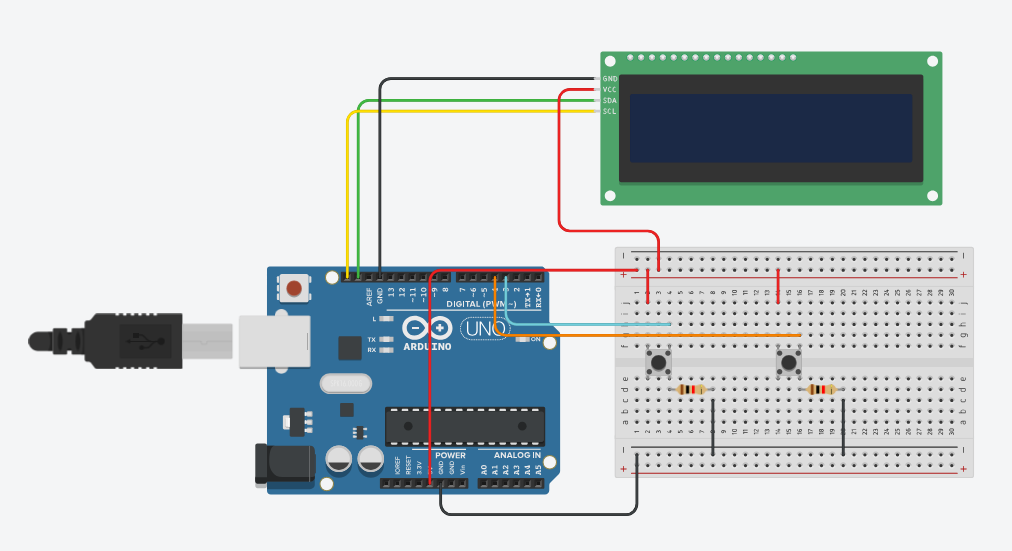
\includegraphics[width=1\linewidth]{CircuitSolved.png}
    \caption{EDEM League electronic table}
    \label{fig:placeholder}
\end{figure}

Based on the provided information and diagram, follow the instructions below to complete the
wiring of the prototype.
\begin{enumerate}
    \item Draw over the diagram the wires needed to connect the circuit (0.5 pts)
    \begin{enumerate}
        \item Complete the variables, constants needed. (0.5 pts)

        \textbf{Solution:}
        We need to add constants for the pins that connect the buttons, and variables to keep track of the amount of points that each team has.
        \begin{verbatim}
            #include <Adafruit_LiquidCrystal.h>
            
            Adafruit_LiquidCrystal lcd(0);
            
            const int B1 = 2;
            const int B2 = 3;
            
            int scoreLocal = 0;
            int scoreVisitor = 0;
        \end{verbatim}
        \item Complete the setup function (1 pts)
        \textbf{Solution:}

        \begin{verbatim}
        void setup() {
          lcd.begin(16, 2);
        
          pinMode(B1, INPUT);
          pinMode(B2, INPUT);
        
          lcd.print("EDEM league");
        }
        \end{verbatim}
    
        \item Complete the loop function (1.5 pts)

        \textbf{Solution:}

        \begin{verbatim}
            void loop() {
              bool b1 = digitalRead(B1);
              bool b2 = digitalRead(B2);
            
              if (b1 == HIGH) {
                scoreLocal += 1;
              }
              if (b2 == HIGH) {
                scoreVisitor += 1;
              }
            
              lcd.setCursor(0, 1);
              lcd.print(scoreLocal);
              lcd.print(" - "); // clear residual digits
              lcd.print(scoreVisitor);
            
              delay(100);
            }
        \end{verbatim}

    \end{enumerate}
\end{enumerate}

To write the code, you can base it on this example of how an LCD screen works, provided as an
example in the next page.

\subsection{Example code}
This code will turn on the LCD screen, write ”hello world” in the first line, and then, in the
second line, it writes, every second, the amount of seconds that it has been working. You can
use this code as inspiration to write the code of the last exercise.

\begin{verbatim}
#include <Adafruit_LiquidCrystal.h>
int seconds = 0;
Adafruit_LiquidCrystal lcd_1(0);
void setup()
{
    lcd_1.begin(16, 2);
    lcd_1.print("hello world");
}
void loop()
{
    lcd_1.setCursor(0, 1);
    lcd_1.print(seconds);
    delay(1000); // Wait for 1000 milliseconds
    seconds += 1;
}    
\end{verbatim}

\section*{Teacher notes and source map}
\subsection*{Preserved source material}
Units 1 (CPU execution) and 3 (Arduino) are reproduced verbatim from \texttt{main.tex} in this directory. This identifies them as Gabriel Modia's units based on the CPU/Python/Arduino division of the supplied exam. No question variants or additional modification tasks have been added.

\subsection*{Scoring in the original}
Unit 1 totals 2 points, although 0.3 is printed twice for the instruction-decoding item. Unit 3 is headed 5 points, but its Q2 heading says 1.5 while its subitems total 3.5. For this rehearsal, use Unit 1 = 2, Unit 2 = 3, Unit 3 Q1 = 1.5 and Q2 = 3.5, for 10 points overall. Count the Unit 1 decoding item once.

\subsection*{Arduino solution qualifications}
The source Q1 asks for nine errors but its solution lists ten; accept any nine as the source specifies. The corrected loop toggles \texttt{pattern} on each iteration where the button reads HIGH, so holding the button can toggle repeatedly. It does not implement one toggle per press.

Similarly, the source Q2 loop increments the score every 100 ms while a button is held. It does not fully implement the stated one-press/one-point requirement. For classroom correction, the implementation below counts a rising edge and assumes ideal, debounced inputs (or a simulator). A real mechanical button also requires debouncing. This is a solution clarification, not an extra student task.
\begin{verbatim}
// Add these variables to the original global declarations:
bool previousB1 = LOW;
bool previousB2 = LOW;

// Replace the original loop with:
void loop() {
    bool b1 = digitalRead(B1);
    bool b2 = digitalRead(B2);
    if (b1 == HIGH && previousB1 == LOW) {
        scoreLocal += 1;
    }
    if (b2 == HIGH && previousB2 == LOW) {
        scoreVisitor += 1;
    }
    previousB1 = b1;
    previousB2 = b2;
    lcd.setCursor(0, 1);
    lcd.print(scoreLocal);
    lcd.print(" - ");
    lcd.print(scoreVisitor);
    lcd.print("   ");
    delay(10);
}
\end{verbatim}
The original \texttt{CircuitSolved.png} supplies the wiring answer. The original LCD example is also retained.
\clearpage\subsection*{Python question sources}
The questions come from the indicated cells. Q3 adds a code template to illustrate the condition, and Q6 explicitly identifies the variables. Q5 uses the prioritisation exercise from Session 06. Original values and answer options are preserved; headings, marks and solutions are added. Cell numbers are one-based and count all notebook cells, including Markdown cells.

\textbf{Q1:} Session 04 - Python execution, functions and libraries -
practice.ipynb --- \textbf{Scenario 4 --- Requesting a concise import},
cells 30.

\textbf{Q2:} Session 05 - Variables, types and numeric operations -
practice.ipynb --- \textbf{Scenario 2 --- Packing devices}, cells 27.

\textbf{Q3:} Session 06 - Boolean expressions and selection control flow
- practice.ipynb --- \textbf{Scenario 4 --- Secure document access},
cells 27.

\textbf{Q4:} Session 08 - Loops, lists and visualisation -
practice.ipynb --- \textbf{B7. Diagnosing an index error}, cells 33.

\textbf{Q5:} Session 06 - Boolean expressions and selection control flow -
practice.ipynb --- \textbf{A7. Prioritise outcomes}, cells 17, 18.

\textbf{Q6:} Session 08 - Loops, lists and visualisation -
practice.ipynb --- \textbf{A5. Preserve a running series}, cells 14, 15.

\end{document}
